\documentclass[a4paper, 12pt, notitlepage]{article}
\usepackage[letterpaper,margin=1in,marginparwidth=1.75cm]{geometry}
\usepackage{graphicx, booktabs, tikz, csquotes, subfig, dcolumn}
\usepackage[font=small,labelfont=bf]{caption}
% \usepackage[markers,figuresonly,nolists]{endfloat}
\usepackage[natbibapa]{apacite}
\usepackage[colorlinks = TRUE, allcolors = blue]{hyperref}
\usepackage[section]{placeins}

\usepackage{setspace}
\setstretch{1.25}

\renewcommand*\rmdefault{ppl}

\title{\Large Online appendix for\\Violence, co-optation, and postwar voting in Guatemala}
\author{}%Francisco Villamil}
\date{}

% Section numbering
\renewcommand{\thesection}{\Alph{section}}

% Table numbering
\renewcommand{\thetable}{A\arabic{table}}

% Table numbering
\renewcommand{\thefigure}{A\arabic{figure}}

\begin{document}

\maketitle

\tableofcontents


\clearpage
\section{Territorial changes in municipalities}\label{app:muni}

A `minimum denomination' of municipalities was built, by joining together those municipalities where changes took place, which consisted mainly of splits.
Thus, if a new municipality was formed out of a bigger one, the two are merged again in the dataset, so as to ensure compatibility between data sources across time.
In particular, the dataset contains observations that range from 1973 to 2015, during which time there has been 15 territorial changes at the local level.
Although one variable goes further back in time, namely rebel activity before 1978, only two territorial changes took place before that date: the formation of Melchor de Mencos (1962) and Poptún (1966).%, both in the department of Petén.
Given that no rebel activity was recorded in the whole territory of Petén before 1971, these two changes were not implemented.
Table \ref{tab:muni} below shows the municipalities that were formed, along with the data and the parent municipality they are merged to in the dataset.

\begin{table}[!htbp] \centering
  \caption{Municipality changes in Guatemala, 1973--2015}
  \label{tab:muni}
  \small
  \begin{tabular}{cccc}
  \\[-1.8ex]\hline
  \hline \\[-1.8ex]
  \\[-1.8ex]
  Department      & New municipality                & Date      & Parent municipality \\
  \hline \\[-1.8ex]
  Alta Verapaz    & Fray Bartolomé de las Casas     & 1980      & Santa María Cahabón \\
  Alta Verapaz    &                    La Tinta     & 1999      &              Panzás \\
  Alta Verapaz    &                     Raxruhá     & 2008      &              Chisec \\
  Escuintla       &            Nueva Concepción     & 1974      &           Tiquisate \\
  Escuintla       &                    Sipacate     & 2015      &           La Gomera \\
  Huehuetenango   &              Unión Cantinil     & 2005      &            Chiantla \\
  Peten           &                     El Chal     & 2014      &             Dolores \\
  Peten           &                  Las Cruces     & 2011      &         La Libertad \\
  Quiche          &                    Chicamán     & 1984      &            Uspantán \\
  Quiche          &                       Ixcán     & 1985      &            Uspantán \\
  Quiche          &                    Pachalúm     & 1986      &             Joyabaj \\
  San Marcos      &                   La Blanca     & 2014      &                Ocós \\
  Suchitepequez   &         San Jose La Maquiná     & 2014      &         Cuyotenango \\
  Zacapa          &                   San Jorge     & 2014      &              Zacapa \\
  \hline
  \hline \\[-1.8ex]
  \end{tabular}
\end{table}

\clearpage
\section{Summary statistics}\label{app:stats}

Table \ref{tab:sumstats}

Figure \ref{fig:corrplot}

\begin{table}[!htbp] \centering
\caption{Summary statistics for the covariates}
\label{tab:sumstats}
\small
\begin{tabular}{lcccccc}
\\[-1.8ex]\hline
\hline \\[-1.8ex]
\\[-1.8ex]
Variable & Min & Q1 & Median & Mean & Q3 & Max \\
\hline \\[-1.8ex]
Log. State killings / 1000hab & 0 & 0 & 0 & 0.63 & 0.66 & 5.36 \\
\% Non-paved roads & 0 & 0.73 & 0.84 & 0.8 & 1 & 1 \\
Log. Distance to PanAm Hwy & 0 & 1.86 & 2.95 & 2.64 & 3.65 & 5.62 \\
Log. Population 1973 & 6.34 & 8.59 & 9.16 & 9.17 & 9.75 & 13.46 \\
\% Indigenous 1973 & 0 & 0.11 & 0.61 & 0.52 & 0.9 & 1 \\
\% Literate 1973 & 0.04 & 0.24 & 0.39 & 0.38 & 0.5 & 0.89 \\
Elevation SD & 4.38 & 140.17 & 224.15 & 262.36 & 351.29 & 764.9 \\
\% Forest cover & 0 & 0.29 & 0.54 & 0.52 & 0.74 & 0.99 \\
Log. distance to capital & 0 & 3.94 & 4.47 & 4.32 & 4.86 & 5.61 \\
Log. Area & 1.53 & 4.06 & 4.88 & 4.88 & 5.52 & 9.01 \\
\hline
\hline \\[-1.8ex]
\end{tabular}
\end{table}



\begin{figure*}[htb!]
  \centering
    \includegraphics[width = 0.7\textwidth]{img/corrplot}

  \caption{Correlation matrix among covariates} \label{fig:corrplot}

\end{figure*}

\clearpage
\section{Accessibility and violence against civilians}\label{app:lm_violence}

Table \ref{tab:lm_govt_vi} shows the results of linear models explaining wartime violence by the state.
Table \ref{tab:lm_govt_vi_hv}


Models in the first two columns run the analyses for the whole sample, including department fixed effects in column 2.
Columns 3 and 4 show equivalent models but restricting the sample to only the most affected departments.

State violence does not have any relevant relationship with the two proxy variables used as interactions.
If anything, it has a positive relationship with the distance to the Pan-American Highway in column 2.
Regarding the other variables, state violence is mainly explained by the share of indigenous population in each municipality and by its size.
When limiting the sample to the most affected departments and including fixed effects, the share of indigenous population stops being significant.

Table \ref{tab:lm_rebels_vi} shows the results for models equivalent to the previous ones but using rebel violence as the dependent variable.
Table \ref{tab:lm_rebels_vi_hv}


Although patterns of rebel violence should not be as relevant to the argument advanced here, it is important to check whether any of the two accessibility proxies is related to local wartime activity.

Again, none of the accessibility proxies shows any relationship to rebel violence.
Rebel violence is also poorly explained by the rest of the variables.
Perhaps because of the relatively low incidence of violence by the rebels, no robust relationship is found.

The results show that the two accessibility variables used as proxies for the level of exposure to prewar mobilization are not related to the intensity of the conflict in each municipality.


% Table created by stargazer v.5.2.2 by Marek Hlavac, Harvard University. E-mail: hlavac at fas.harvard.edu
% Date and time: Fri, Jul 02, 2021 - 12:56:13
% Requires LaTeX packages: dcolumn 
\begin{table}[!htbp] \centering 
  \caption{Determinants of wartime violence by the state} 
  \label{tab:lm_govt_vi} 
\small 
\begin{tabular}{@{\extracolsep{-20pt}}lD{.}{.}{-3} D{.}{.}{-3} D{.}{.}{-3} D{.}{.}{-3} } 
\\[-1.8ex]\hline 
\hline \\[-1.8ex] 
\\[-1.8ex] & \multicolumn{1}{c}{(1)} & \multicolumn{1}{c}{(2)} & \multicolumn{1}{c}{(3)} & \multicolumn{1}{c}{(4)}\\ 
\hline \\[-1.8ex] 
 (Intercept) & -0.250 & 1.208^{**} & -0.196 & -0.185 \\ 
  & (0.261) & (0.394) & (0.915) & (1.217) \\ 
  \% Roads non-paved & 0.900^{**} & -0.139 & -0.169 & -0.328 \\ 
  & (0.314) & (0.263) & (0.309) & (0.273) \\ 
  Log. Distance to Pan-Am Hwy & 0.062 & 0.089 & -0.026 & 0.101^{+} \\ 
  & (0.046) & (0.056) & (0.049) & (0.058) \\ 
  Log. Population 1973 &  &  & -0.110 & 0.030 \\ 
  &  &  & (0.085) & (0.085) \\ 
  \% Indigenous 1973 &  &  & 1.130^{***} & 0.487^{+} \\ 
  &  &  & (0.229) & (0.262) \\ 
  \% Literate 1973 &  &  & -0.901^{+} & 0.177 \\ 
  &  &  & (0.485) & (0.489) \\ 
  Elevation SD &  &  & -0.000 & -0.000 \\ 
  &  &  & (0.000) & (0.000) \\ 
  Forest cover &  &  & 0.211 & 0.216 \\ 
  &  &  & (0.274) & (0.253) \\ 
  Log. Dist to capital &  &  & -0.071 & -0.208 \\ 
  &  &  & (0.094) & (0.201) \\ 
  Log. Area &  &  & 0.422^{***} & 0.271^{**} \\ 
  &  &  & (0.070) & (0.083) \\ 
  Rebel violence pre-78 &  &  & 2.053 & 2.080 \\ 
  &  &  & (1.553) & (1.300) \\ 
 \hline \\[-1.8ex] 
Department FE & \multicolumn{1}{c}{No} & \multicolumn{1}{c}{Yes} & \multicolumn{1}{c}{No} & \multicolumn{1}{c}{Yes} \\ 
Observations & \multicolumn{1}{c}{325} & \multicolumn{1}{c}{325} & \multicolumn{1}{c}{325} & \multicolumn{1}{c}{325} \\ 
R$^{2}$ & \multicolumn{1}{c}{0.037} & \multicolumn{1}{c}{0.529} & \multicolumn{1}{c}{0.285} & \multicolumn{1}{c}{0.575} \\ 
Adjusted R$^{2}$ & \multicolumn{1}{c}{0.031} & \multicolumn{1}{c}{0.493} & \multicolumn{1}{c}{0.262} & \multicolumn{1}{c}{0.530} \\ 
\hline 
\hline \\[-1.8ex] 
\multicolumn{5}{c}{\parbox[t]{0.65\textwidth}{\textit{Note:} $+ p<0.1; * p<0.05; ** p<0.01; *** p<0.001$. Department FEs not shown.}} \\ 
\end{tabular} 
\end{table} 


% Table created by stargazer v.5.2.2 by Marek Hlavac, Harvard University. E-mail: hlavac at fas.harvard.edu
% Date and time: Thu, Jul 15, 2021 - 11:05:11
% Requires LaTeX packages: dcolumn 
\begin{table}[!htbp] \centering 
  \caption{Determinants of wartime violence by the state (most affected departments)} 
  \label{tab:lm_govt_vi_hv} 
\small 
\begin{tabular}{@{\extracolsep{-20pt}}lD{.}{.}{-3} D{.}{.}{-3} D{.}{.}{-3} D{.}{.}{-3} } 
\\[-1.8ex]\hline 
\hline \\[-1.8ex] 
\\[-1.8ex] & \multicolumn{1}{c}{(1)} & \multicolumn{1}{c}{(2)} & \multicolumn{1}{c}{(3)} & \multicolumn{1}{c}{(4)}\\ 
\hline \\[-1.8ex] 
 (Intercept) & 1.524 & 1.008 & -3.137 & -3.999 \\ 
  & (1.059) & (1.159) & (2.926) & (4.097) \\ 
  \% Roads non-paved & -0.003 & -0.783 & 0.114 & -0.947 \\ 
  & (1.256) & (1.386) & (1.461) & (1.382) \\ 
  Log. Distance to Pan-Am Hwy & 0.091 & 0.266 & 0.043 & 0.190 \\ 
  & (0.099) & (0.171) & (0.135) & (0.169) \\ 
  Log. Population 1973 &  &  & 0.473^{+} & 0.333 \\ 
  &  &  & (0.257) & (0.252) \\ 
  \% Indigenous 1973 &  &  & 0.783 & 1.069 \\ 
  &  &  & (0.828) & (0.855) \\ 
  \% Literate 1973 &  &  & -1.052 & 1.279 \\ 
  &  &  & (1.383) & (1.583) \\ 
  Elevation SD &  &  & -0.001 & -0.002 \\ 
  &  &  & (0.001) & (0.001) \\ 
  Forest cover &  &  & -1.154 & 0.422 \\ 
  &  &  & (0.720) & (0.741) \\ 
  Log. Dist to capital &  &  & -0.206 & -0.511 \\ 
  &  &  & (0.302) & (0.748) \\ 
  Log. Area &  &  & 0.373^{+} & 0.601^{**} \\ 
  &  &  & (0.198) & (0.212) \\ 
  Rebel violence pre-78 &  &  & 5.043 & 3.329 \\ 
  &  &  & (6.798) & (6.325) \\ 
 \hline \\[-1.8ex] 
Department FE & \multicolumn{1}{c}{No} & \multicolumn{1}{c}{Yes} & \multicolumn{1}{c}{No} & \multicolumn{1}{c}{Yes} \\ 
Observations & \multicolumn{1}{c}{99} & \multicolumn{1}{c}{99} & \multicolumn{1}{c}{99} & \multicolumn{1}{c}{99} \\ 
R$^{2}$ & \multicolumn{1}{c}{0.010} & \multicolumn{1}{c}{0.242} & \multicolumn{1}{c}{0.234} & \multicolumn{1}{c}{0.412} \\ 
Adjusted R$^{2}$ & \multicolumn{1}{c}{-0.010} & \multicolumn{1}{c}{0.183} & \multicolumn{1}{c}{0.147} & \multicolumn{1}{c}{0.305} \\ 
\hline 
\hline \\[-1.8ex] 
\multicolumn{5}{c}{\parbox[t]{0.65\textwidth}{\textit{Note:} $+ p<0.1; * p<0.05; ** p<0.01; *** p<0.001$. Department FEs not shown. Most affected departments include Huehuetenango, Chimaltenango, Quiché, Alta Verapaz, Baja Verapaz, and Petén.}} \\ 
\end{tabular} 
\end{table} 


% Table created by stargazer v.5.2.2 by Marek Hlavac, Harvard University. E-mail: hlavac at fas.harvard.edu
% Date and time: Fri, Oct 29, 2021 - 20:43:38
% Requires LaTeX packages: dcolumn 
\begin{table}[!htbp] \centering 
  \caption{Determinants of wartime violence by the rebels} 
  \label{tab:lm_rebels_vi} 
\small 
\begin{tabular}{@{\extracolsep{-20pt}}lD{.}{.}{-3} D{.}{.}{-3} D{.}{.}{-3} D{.}{.}{-3} } 
\\[-1.8ex]\hline 
\hline \\[-1.8ex] 
\\[-1.8ex] & \multicolumn{1}{c}{(1)} & \multicolumn{1}{c}{(2)} & \multicolumn{1}{c}{(3)} & \multicolumn{1}{c}{(4)}\\ 
\hline \\[-1.8ex] 
 (Intercept) & -0.021 & -0.049 & 0.031 & -0.276 \\ 
  & (0.038) & (0.080) & (0.153) & (0.257) \\ 
  \% Roads non-paved & 0.024 & -0.005 & -0.043 & -0.048 \\ 
  & (0.046) & (0.054) & (0.052) & (0.058) \\ 
  Log. Distance to Pan-Am Hwy & 0.011 & 0.012 & 0.003 & 0.006 \\ 
  & (0.007) & (0.011) & (0.008) & (0.012) \\ 
  Log. Population 1973 &  &  & -0.017 & -0.009 \\ 
  &  &  & (0.014) & (0.018) \\ 
  \% Indigenous 1973 &  &  & 0.057 & 0.016 \\ 
  &  &  & (0.038) & (0.055) \\ 
  \% Literate 1973 &  &  & -0.006 & -0.024 \\ 
  &  &  & (0.081) & (0.103) \\ 
  Elevation SD &  &  & 0.000 & 0.000 \\ 
  &  &  & (0.000) & (0.000) \\ 
  Forest cover &  &  & -0.028 & 0.012 \\ 
  &  &  & (0.046) & (0.053) \\ 
  Log. Dist to capital &  &  & -0.002 & 0.034 \\ 
  &  &  & (0.016) & (0.042) \\ 
  Log. Area &  &  & 0.034^{**} & 0.034^{+} \\ 
  &  &  & (0.012) & (0.018) \\ 
  Rebel violence pre-78 &  &  & 0.138 & 0.196 \\ 
  &  &  & (0.260) & (0.275) \\ 
 \hline \\[-1.8ex] 
Department FE & \multicolumn{1}{c}{No} & \multicolumn{1}{c}{Yes} & \multicolumn{1}{c}{No} & \multicolumn{1}{c}{Yes} \\ 
Observations & \multicolumn{1}{c}{325} & \multicolumn{1}{c}{325} & \multicolumn{1}{c}{325} & \multicolumn{1}{c}{325} \\ 
R$^{2}$ & \multicolumn{1}{c}{0.010} & \multicolumn{1}{c}{0.070} & \multicolumn{1}{c}{0.046} & \multicolumn{1}{c}{0.097} \\ 
Adjusted R$^{2}$ & \multicolumn{1}{c}{0.004} & \multicolumn{1}{c}{-0.002} & \multicolumn{1}{c}{0.016} & \multicolumn{1}{c}{0.002} \\ 
\hline 
\hline \\[-1.8ex] 
\multicolumn{5}{c}{\parbox[t]{0.65\textwidth}{\textit{Note:} $+ p<0.1; * p<0.05; ** p<0.01; *** p<0.001$. Department FEs not shown.}} \\ 
\end{tabular} 
\end{table} 

\input{tab/tab_rebels_vi_hv.tex}

\clearpage
\section{Full tables (main text)}\label{app:results_tablong}


% Table created by stargazer v.5.2.2 by Marek Hlavac, Harvard University. E-mail: hlavac at fas.harvard.edu
% Date and time: Wed, May 19, 2021 - 10:03:17
% Requires LaTeX packages: dcolumn 
\begin{table}[!htbp] \centering 
  \caption{Base models on wartime violence and postwar voting} 
  \label{tab:lm_base} 
\small 
\begin{tabular}{@{\extracolsep{-20pt}}lD{.}{.}{-3} D{.}{.}{-3} D{.}{.}{-3} D{.}{.}{-3} } 
\\[-1.8ex]\hline 
\hline \\[-1.8ex] 
\\[-1.8ex] & \multicolumn{1}{c}{URNG} & \multicolumn{1}{c}{FRG} & \multicolumn{1}{c}{URNG} & \multicolumn{1}{c}{FRG} \\ 
 & \multicolumn{2}{c}{} & \multicolumn{2}{c}{\scriptsize Most affected departments} \\ 
\\[-1.8ex] & \multicolumn{1}{c}{(1)} & \multicolumn{1}{c}{(2)} & \multicolumn{1}{c}{(3)} & \multicolumn{1}{c}{(4)}\\ 
\hline \\[-1.8ex] 
 (Intercept) & 0.000 & 0.511^{***} & 0.021 & 0.448^{**} \\ 
  & (0.039) & (0.067) & (0.101) & (0.167) \\ 
  State-led killings & 0.007^{***} & -0.001 & 0.005^{+} & 0.001 \\ 
  & (0.002) & (0.003) & (0.003) & (0.004) \\ 
  Log. Population 1973 & 0.006^{*} & -0.002 & 0.001 & 0.005 \\ 
  & (0.003) & (0.005) & (0.006) & (0.010) \\ 
  \% Indigenous 1973 & 0.035^{***} & -0.014 & 0.043^{*} & -0.021 \\ 
  & (0.008) & (0.014) & (0.021) & (0.035) \\ 
  \% Literate 1973 & -0.040^{*} & 0.002 & -0.046 & 0.087 \\ 
  & (0.016) & (0.027) & (0.039) & (0.064) \\ 
  Elevation SD & -0.000^{+} & -0.000 & -0.000^{*} & 0.000 \\ 
  & (0.000) & (0.000) & (0.000) & (0.000) \\ 
  Forest cover & 0.016^{*} & -0.022 & 0.042^{*} & -0.032 \\ 
  & (0.008) & (0.014) & (0.018) & (0.030) \\ 
  Log. Dist to capital & 0.004 & 0.006 & 0.008 & 0.002 \\ 
  & (0.006) & (0.010) & (0.018) & (0.030) \\ 
  Log. Area & 0.005^{*} & 0.004 & 0.007 & -0.003 \\ 
  & (0.003) & (0.004) & (0.005) & (0.009) \\ 
  Rebel violence pre-78 & 0.011 & 0.015 & -0.054 & -0.027 \\ 
  & (0.041) & (0.071) & (0.156) & (0.258) \\ 
 \hline \\[-1.8ex] 
Department FE & \multicolumn{1}{c}{Yes} & \multicolumn{1}{c}{Yes} & \multicolumn{1}{c}{Yes} & \multicolumn{1}{c}{Yes} \\ 
Election FE & \multicolumn{1}{c}{Yes} & \multicolumn{1}{c}{Yes} & \multicolumn{1}{c}{Yes} & \multicolumn{1}{c}{Yes} \\ 
Observations & \multicolumn{1}{c}{1,601} & \multicolumn{1}{c}{1,281} & \multicolumn{1}{c}{491} & \multicolumn{1}{c}{394} \\ 
R$^{2}$ & \multicolumn{1}{c}{0.442} & \multicolumn{1}{c}{0.814} & \multicolumn{1}{c}{0.387} & \multicolumn{1}{c}{0.731} \\ 
Adjusted R$^{2}$ & \multicolumn{1}{c}{0.430} & \multicolumn{1}{c}{0.809} & \multicolumn{1}{c}{0.364} & \multicolumn{1}{c}{0.719} \\ 
\hline 
\hline \\[-1.8ex] 
\multicolumn{5}{c}{\parbox[t]{0.65\textwidth}{\textit{Note:} $+ p<0.1; * p<0.05; ** p<0.01; *** p<0.001$. All models pool all observations across all elections. Election and department FEs not shown. Most affected departments include Huehuetenango, Chimaltenango, Quiché, Alta Verapaz, Baja Verapaz, and Petén.}} \\ 
\end{tabular} 
\end{table} 



% Table created by stargazer v.5.2.2 by Marek Hlavac, Harvard University. E-mail: hlavac at fas.harvard.edu
% Date and time: Tue, May 18, 2021 - 13:01:58
% Requires LaTeX packages: dcolumn 
\begin{table}[!htbp] \centering 
  \caption{Wartime violence, local road network, and voting} 
  \label{tab:lm_roads} 
\small 
\begin{tabular}{@{\extracolsep{-20pt}}lD{.}{.}{-3} D{.}{.}{-3} D{.}{.}{-3} D{.}{.}{-3} } 
\\[-1.8ex]\hline 
\hline \\[-1.8ex] 
\\[-1.8ex] & \multicolumn{1}{c}{URNG} & \multicolumn{1}{c}{FRG} & \multicolumn{1}{c}{URNG} & \multicolumn{1}{c}{FRG} \\ 
 & \multicolumn{2}{c}{} & \multicolumn{2}{c}{\scriptsize Most affected departments} \\ 
\\[-1.8ex] & \multicolumn{1}{c}{(1)} & \multicolumn{1}{c}{(2)} & \multicolumn{1}{c}{(3)} & \multicolumn{1}{c}{(4)}\\ 
\hline \\[-1.8ex] 
 (Intercept) & -0.032 & 0.530^{***} & -0.158 & 0.602^{***} \\ 
  & (0.039) & (0.068) & (0.108) & (0.181) \\ 
  State-led killings & 0.044^{***} & -0.031^{*} & 0.081^{***} & -0.069^{*} \\ 
  & (0.007) & (0.013) & (0.017) & (0.028) \\ 
  \% Non-paved roads & 0.004 & 0.009 & 0.078^{*} & -0.042 \\ 
  & (0.009) & (0.016) & (0.038) & (0.064) \\ 
  Violence $\times$ Non-paved & -0.043^{***} & 0.034^{*} & -0.084^{***} & 0.077^{*} \\ 
  & (0.008) & (0.014) & (0.018) & (0.030) \\ 
  Log. Population 1973 & 0.006^{*} & -0.001 & 0.001 & 0.006 \\ 
  & (0.003) & (0.005) & (0.006) & (0.010) \\ 
  \% Indigenous 1973 & 0.038^{***} & -0.018 & 0.050^{*} & -0.029 \\ 
  & (0.008) & (0.014) & (0.021) & (0.035) \\ 
  \% Literate 1973 & -0.030^{+} & -0.007 & -0.025 & 0.062 \\ 
  & (0.016) & (0.027) & (0.039) & (0.064) \\ 
  Elevation SD & -0.000 & -0.000 & -0.000 & -0.000 \\ 
  & (0.000) & (0.000) & (0.000) & (0.000) \\ 
  Forest cover & 0.014^{+} & -0.021 & 0.033^{+} & -0.024 \\ 
  & (0.008) & (0.014) & (0.018) & (0.030) \\ 
  Log. Dist to capital & 0.008 & 0.001 & 0.028 & -0.019 \\ 
  & (0.006) & (0.011) & (0.019) & (0.031) \\ 
  Log. Area & 0.006^{*} & 0.003 & 0.007 & -0.003 \\ 
  & (0.003) & (0.005) & (0.005) & (0.009) \\ 
  Rebel violence pre-78 & 0.007 & 0.019 & -0.026 & -0.062 \\ 
  & (0.041) & (0.071) & (0.153) & (0.256) \\ 
 \hline \\[-1.8ex] 
Department FE & \multicolumn{1}{c}{Yes} & \multicolumn{1}{c}{Yes} & \multicolumn{1}{c}{Yes} & \multicolumn{1}{c}{Yes} \\ 
Election FE & \multicolumn{1}{c}{Yes} & \multicolumn{1}{c}{Yes} & \multicolumn{1}{c}{Yes} & \multicolumn{1}{c}{Yes} \\ 
Observations & \multicolumn{1}{c}{1,601} & \multicolumn{1}{c}{1,281} & \multicolumn{1}{c}{491} & \multicolumn{1}{c}{394} \\ 
R$^{2}$ & \multicolumn{1}{c}{0.453} & \multicolumn{1}{c}{0.815} & \multicolumn{1}{c}{0.415} & \multicolumn{1}{c}{0.737} \\ 
Adjusted R$^{2}$ & \multicolumn{1}{c}{0.440} & \multicolumn{1}{c}{0.810} & \multicolumn{1}{c}{0.390} & \multicolumn{1}{c}{0.723} \\ 
\hline 
\hline \\[-1.8ex] 
\multicolumn{5}{c}{\parbox[t]{0.65\textwidth}{\textit{Note:} $+ p<0.1; * p<0.05; ** p<0.01; *** p<0.001$. All models pool all observations across all elections. Election and department FEs not shown. Most affected departments include Huehuetenango, Chimaltenango, Quiché, Alta Verapaz, Baja Verapaz, and Petén.}} \\ 
\end{tabular} 
\end{table} 



% Table created by stargazer v.5.2.2 by Marek Hlavac, Harvard University. E-mail: hlavac at fas.harvard.edu
% Date and time: Tue, Jul 27, 2021 - 13:56:47
% Requires LaTeX packages: dcolumn 
\begin{table}[!htbp] \centering 
  \caption{Wartime violence, distance to PanAm Highway, and voting} 
  \label{tab:lm_panam} 
\small 
\begin{tabular}{@{\extracolsep{-20pt}}lD{.}{.}{-3} D{.}{.}{-3} D{.}{.}{-3} D{.}{.}{-3} } 
\\[-1.8ex]\hline 
\hline \\[-1.8ex] 
\\[-1.8ex] & \multicolumn{1}{c}{URNG} & \multicolumn{1}{c}{FRG} & \multicolumn{1}{c}{URNG} & \multicolumn{1}{c}{FRG} \\ 
 & \multicolumn{2}{c}{} & \multicolumn{2}{c}{\scriptsize Most affected departments} \\ 
\\[-1.8ex] & \multicolumn{1}{c}{(1)} & \multicolumn{1}{c}{(2)} & \multicolumn{1}{c}{(3)} & \multicolumn{1}{c}{(4)}\\ 
\hline \\[-1.8ex] 
 (Intercept) & 0.015 & 0.506^{***} & 0.052 & 0.433^{*} \\ 
  & (0.038) & (0.067) & (0.100) & (0.168) \\ 
  State-led killings & 0.024^{***} & -0.004 & 0.022^{***} & -0.003 \\ 
  & (0.004) & (0.006) & (0.005) & (0.009) \\ 
  Log. Dist to Pan-Am Hwy & 0.001 & 0.004 & 0.001 & 0.004 \\ 
  & (0.002) & (0.003) & (0.004) & (0.007) \\ 
  Violence $\times$ Dist to Pan-Am & -0.006^{***} & 0.001 & -0.006^{***} & 0.001 \\ 
  & (0.001) & (0.002) & (0.002) & (0.003) \\ 
  Log. Population 1973 & 0.003 & -0.001 & -0.006 & 0.008 \\ 
  & (0.003) & (0.005) & (0.006) & (0.011) \\ 
  \% Indigenous 1973 & 0.037^{***} & -0.013 & 0.043^{*} & -0.024 \\ 
  & (0.008) & (0.014) & (0.021) & (0.035) \\ 
  \% Literate 1973 & -0.035^{*} & 0.003 & -0.046 & 0.082 \\ 
  & (0.015) & (0.027) & (0.039) & (0.064) \\ 
  Elevation SD & -0.000 & -0.000 & -0.000 & -0.000 \\ 
  & (0.000) & (0.000) & (0.000) & (0.000) \\ 
  Forest cover & 0.014^{+} & -0.024^{+} & 0.038^{*} & -0.034 \\ 
  & (0.008) & (0.014) & (0.018) & (0.031) \\ 
  Log. Dist to capital & 0.004 & 0.001 & 0.009 & 0.000 \\ 
  & (0.006) & (0.011) & (0.018) & (0.030) \\ 
  Log. Area & 0.007^{**} & 0.003 & 0.012^{*} & -0.004 \\ 
  & (0.003) & (0.005) & (0.005) & (0.009) \\ 
  Rebel violence pre-78 & 0.020 & 0.011 & -0.019 & -0.037 \\ 
  & (0.041) & (0.071) & (0.154) & (0.259) \\ 
 \hline \\[-1.8ex] 
Department FE & \multicolumn{1}{c}{Yes} & \multicolumn{1}{c}{Yes} & \multicolumn{1}{c}{Yes} & \multicolumn{1}{c}{Yes} \\ 
Election FE & \multicolumn{1}{c}{Yes} & \multicolumn{1}{c}{Yes} & \multicolumn{1}{c}{Yes} & \multicolumn{1}{c}{Yes} \\ 
Observations & \multicolumn{1}{c}{1,601} & \multicolumn{1}{c}{1,281} & \multicolumn{1}{c}{491} & \multicolumn{1}{c}{394} \\ 
R$^{2}$ & \multicolumn{1}{c}{0.453} & \multicolumn{1}{c}{0.814} & \multicolumn{1}{c}{0.407} & \multicolumn{1}{c}{0.732} \\ 
Adjusted R$^{2}$ & \multicolumn{1}{c}{0.441} & \multicolumn{1}{c}{0.809} & \multicolumn{1}{c}{0.382} & \multicolumn{1}{c}{0.718} \\ 
\hline 
\hline \\[-1.8ex] 
\multicolumn{5}{c}{\parbox[t]{0.65\textwidth}{\textit{Note:} $+ p<0.1; * p<0.05; ** p<0.01; *** p<0.001$. All models pool all observations across all elections. Election and department FEs not shown. Most affected departments include Huehuetenango, Chimaltenango, Quiché, Alta Verapaz, Baja Verapaz, and Petén.}} \\ 
\end{tabular} 
\end{table} 


\clearpage
\section{Results using only CEH data for violence variables}\label{app:results_ceh}

Tables \ref{tab:lm_roads_ceh} and \ref{tab:lm_panam_ceh} replicate the main results using only CEH data to measure wartime violence.


% Table created by stargazer v.5.2.2 by Marek Hlavac, Harvard University. E-mail: hlavac at fas.harvard.edu
% Date and time: Mon, Jul 26, 2021 - 13:55:22
% Requires LaTeX packages: dcolumn 
\begin{table}[!htbp] \centering 
  \caption{Wartime violence (using only CEH), local road network, and voting} 
  \label{tab:lm_roads_ceh} 
\small 
\begin{tabular}{@{\extracolsep{-20pt}}lD{.}{.}{-3} D{.}{.}{-3} D{.}{.}{-3} D{.}{.}{-3} } 
\\[-1.8ex]\hline 
\hline \\[-1.8ex] 
\\[-1.8ex] & \multicolumn{1}{c}{URNG} & \multicolumn{1}{c}{FRG} & \multicolumn{1}{c}{URNG} & \multicolumn{1}{c}{FRG} \\ 
 & \multicolumn{2}{c}{} & \multicolumn{2}{c}{\scriptsize Most affected departments} \\ 
\\[-1.8ex] & \multicolumn{1}{c}{(1)} & \multicolumn{1}{c}{(2)} & \multicolumn{1}{c}{(3)} & \multicolumn{1}{c}{(4)}\\ 
\hline \\[-1.8ex] 
 (Intercept) & -0.029 & 0.516^{***} & -0.072 & 0.548^{**} \\ 
  & (0.038) & (0.066) & (0.106) & (0.178) \\ 
  State-led killings & 0.050^{***} & -0.028^{+} & 0.077^{***} & -0.054^{+} \\ 
  & (0.009) & (0.015) & (0.018) & (0.030) \\ 
  \% Non-paved roads & -0.001 & 0.013 & 0.024 & 0.017 \\ 
  & (0.009) & (0.015) & (0.034) & (0.058) \\ 
  Violence $\times$ Non-paved & -0.047^{***} & 0.031^{+} & -0.077^{***} & 0.061^{+} \\ 
  & (0.010) & (0.017) & (0.020) & (0.033) \\ 
  Log. Population 1973 & 0.004 & -0.001 & -0.000 & 0.007 \\ 
  & (0.003) & (0.005) & (0.006) & (0.010) \\ 
  \% Indigenous 1973 & 0.047^{***} & -0.016 & 0.053^{***} & -0.050^{+} \\ 
  & (0.007) & (0.012) & (0.015) & (0.026) \\ 
  \% Literate 1973 & -0.000 & -0.000 & -0.000 & -0.000 \\ 
  & (0.000) & (0.000) & (0.000) & (0.000) \\ 
  Elevation SD & 0.014^{+} & -0.021 & 0.034^{+} & -0.035 \\ 
  & (0.008) & (0.014) & (0.018) & (0.030) \\ 
  Forest cover & 0.006 & 0.002 & 0.017 & -0.009 \\ 
  & (0.006) & (0.011) & (0.018) & (0.031) \\ 
  Log. Dist to capital & 0.007^{**} & 0.002 & 0.009^{+} & -0.007 \\ 
  & (0.003) & (0.004) & (0.005) & (0.009) \\ 
  Log. Area & 0.017 & 0.014 & -0.045 & -0.011 \\ 
  & (0.041) & (0.071) & (0.154) & (0.258) \\ 
 \hline \\[-1.8ex] 
Department FE & \multicolumn{1}{c}{Yes} & \multicolumn{1}{c}{Yes} & \multicolumn{1}{c}{Yes} & \multicolumn{1}{c}{Yes} \\ 
Election FE & \multicolumn{1}{c}{Yes} & \multicolumn{1}{c}{Yes} & \multicolumn{1}{c}{Yes} & \multicolumn{1}{c}{Yes} \\ 
Observations & \multicolumn{1}{c}{1,601} & \multicolumn{1}{c}{1,281} & \multicolumn{1}{c}{491} & \multicolumn{1}{c}{394} \\ 
R$^{2}$ & \multicolumn{1}{c}{0.451} & \multicolumn{1}{c}{0.815} & \multicolumn{1}{c}{0.410} & \multicolumn{1}{c}{0.734} \\ 
Adjusted R$^{2}$ & \multicolumn{1}{c}{0.438} & \multicolumn{1}{c}{0.809} & \multicolumn{1}{c}{0.387} & \multicolumn{1}{c}{0.721} \\ 
\hline 
\hline \\[-1.8ex] 
\multicolumn{5}{c}{\parbox[t]{0.65\textwidth}{\textit{Note:} $+ p<0.1; * p<0.05; ** p<0.01; *** p<0.001$. All models pool all observations across all elections. Election and department FEs not shown. Most affected departments include Huehuetenango, Chimaltenango, Quiché, Alta Verapaz, Baja Verapaz, and Petén.}} \\ 
\end{tabular} 
\end{table} 


% Table created by stargazer v.5.2.2 by Marek Hlavac, Harvard University. E-mail: hlavac at fas.harvard.edu
% Date and time: Mon, Jul 26, 2021 - 13:55:22
% Requires LaTeX packages: dcolumn 
\begin{table}[!htbp] \centering 
  \caption{Wartime violence (using only CEH), distance to PanAm Hwy, and voting} 
  \label{tab:lm_panam_ceh} 
\small 
\begin{tabular}{@{\extracolsep{-20pt}}lD{.}{.}{-3} D{.}{.}{-3} D{.}{.}{-3} D{.}{.}{-3} } 
\\[-1.8ex]\hline 
\hline \\[-1.8ex] 
\\[-1.8ex] & \multicolumn{1}{c}{URNG} & \multicolumn{1}{c}{FRG} & \multicolumn{1}{c}{URNG} & \multicolumn{1}{c}{FRG} \\ 
 & \multicolumn{2}{c}{} & \multicolumn{2}{c}{\scriptsize Most affected departments} \\ 
\\[-1.8ex] & \multicolumn{1}{c}{(1)} & \multicolumn{1}{c}{(2)} & \multicolumn{1}{c}{(3)} & \multicolumn{1}{c}{(4)}\\ 
\hline \\[-1.8ex] 
 (Intercept) & 0.012 & 0.509^{***} & 0.071 & 0.458^{**} \\ 
  & (0.038) & (0.065) & (0.101) & (0.170) \\ 
  State-led killings & 0.031^{***} & -0.000 & 0.030^{***} & 0.004 \\ 
  & (0.004) & (0.007) & (0.006) & (0.011) \\ 
  Log. Dist to Pan-Am Hwy & 0.001 & 0.005 & 0.001 & 0.007 \\ 
  & (0.002) & (0.003) & (0.004) & (0.007) \\ 
  Violence $\times$ Dist to Pan-Am & -0.007^{***} & -0.001 & -0.007^{***} & -0.001 \\ 
  & (0.001) & (0.002) & (0.002) & (0.003) \\ 
  Log. Population 1973 & 0.002 & -0.001 & -0.007 & 0.008 \\ 
  & (0.003) & (0.005) & (0.006) & (0.010) \\ 
  \% Indigenous 1973 & 0.045^{***} & -0.014 & 0.052^{***} & -0.056^{*} \\ 
  & (0.007) & (0.011) & (0.015) & (0.026) \\ 
  \% Literate 1973 & -0.000 & -0.000 & -0.000 & -0.000 \\ 
  & (0.000) & (0.000) & (0.000) & (0.000) \\ 
  Elevation SD & 0.012 & -0.024^{+} & 0.032^{+} & -0.044 \\ 
  & (0.008) & (0.014) & (0.018) & (0.031) \\ 
  Forest cover & 0.002 & 0.001 & 0.004 & 0.006 \\ 
  & (0.006) & (0.011) & (0.018) & (0.030) \\ 
  Log. Dist to capital & 0.009^{***} & 0.004 & 0.012^{*} & -0.007 \\ 
  & (0.003) & (0.004) & (0.005) & (0.009) \\ 
  Log. Area & 0.013 & 0.008 & -0.021 & -0.027 \\ 
  & (0.041) & (0.071) & (0.153) & (0.258) \\ 
 \hline \\[-1.8ex] 
Department FE & \multicolumn{1}{c}{Yes} & \multicolumn{1}{c}{Yes} & \multicolumn{1}{c}{Yes} & \multicolumn{1}{c}{Yes} \\ 
Election FE & \multicolumn{1}{c}{Yes} & \multicolumn{1}{c}{Yes} & \multicolumn{1}{c}{Yes} & \multicolumn{1}{c}{Yes} \\ 
Observations & \multicolumn{1}{c}{1,601} & \multicolumn{1}{c}{1,281} & \multicolumn{1}{c}{491} & \multicolumn{1}{c}{394} \\ 
R$^{2}$ & \multicolumn{1}{c}{0.454} & \multicolumn{1}{c}{0.814} & \multicolumn{1}{c}{0.413} & \multicolumn{1}{c}{0.731} \\ 
Adjusted R$^{2}$ & \multicolumn{1}{c}{0.442} & \multicolumn{1}{c}{0.809} & \multicolumn{1}{c}{0.389} & \multicolumn{1}{c}{0.718} \\ 
\hline 
\hline \\[-1.8ex] 
\multicolumn{5}{c}{\parbox[t]{0.65\textwidth}{\textit{Note:} $+ p<0.1; * p<0.05; ** p<0.01; *** p<0.001$. All models pool all observations across all elections. Election and department FEs not shown. Most affected departments include Huehuetenango, Chimaltenango, Quiché, Alta Verapaz, Baja Verapaz, and Petén.}} \\ 
\end{tabular} 
\end{table} 


\clearpage
\section{Results aggregating several parties}\label{app:results_full}

Table \ref{tab:lm_fulldcha}
Table \ref{tab:lm_fullizq}

Figure \ref{fig:pp_fulldcha_roads}
Figure \ref{fig:pp_fulldcha_panam}
Figure \ref{fig:pp_fullizq_roads}
Figure \ref{fig:pp_fullizq_panam}


% Table created by stargazer v.5.2.2 by Marek Hlavac, Harvard University. E-mail: hlavac at fas.harvard.edu
% Date and time: Mon, Jul 26, 2021 - 13:55:22
% Requires LaTeX packages: dcolumn 
\begin{table}[!htbp] \centering 
  \caption{Wartime violence, prewar mobilization, and voting for FRG, Partido Patriota, and FCN} 
  \label{tab:lm_fulldcha} 
\small 
\begin{tabular}{@{\extracolsep{-20pt}}lD{.}{.}{-3} D{.}{.}{-3} D{.}{.}{-3} D{.}{.}{-3} } 
\\[-1.8ex]\hline 
\hline \\[-1.8ex] 
\\[-1.8ex] & \multicolumn{1}{c}{} & \multicolumn{1}{c}{} & \multicolumn{1}{c}{} & \multicolumn{1}{c}{} \\ 
 & \multicolumn{2}{c}{} & \multicolumn{2}{c}{\scriptsize Most affected departments} \\ 
\\[-1.8ex] & \multicolumn{1}{c}{(1)} & \multicolumn{1}{c}{(2)} & \multicolumn{1}{c}{(3)} & \multicolumn{1}{c}{(4)}\\ 
\hline \\[-1.8ex] 
 (Intercept) & 0.573^{***} & 0.525^{***} & 0.958^{***} & 0.660^{***} \\ 
  & (0.076) & (0.074) & (0.196) & (0.183) \\ 
  State-led killings & -0.047^{**} & -0.019^{**} & -0.109^{***} & -0.013 \\ 
  & (0.014) & (0.007) & (0.030) & (0.010) \\ 
  \% Non-paved roads & -0.004 &  & -0.132^{+} &  \\ 
  & (0.017) &  & (0.070) &  \\ 
  Violence $\times$ Non-paved & 0.051^{**} &  & 0.121^{***} &  \\ 
  & (0.016) &  & (0.033) &  \\ 
  Log. Dist to Pan-Am Hwy &  & -0.006 &  & 0.002 \\ 
  &  & (0.004) &  & (0.008) \\ 
  Violence $\times$ Dist to Pan-Am &  & 0.006^{**} &  & 0.004 \\ 
  &  & (0.002) &  & (0.003) \\ 
  Log. Population 1973 & 0.000 & 0.002 & -0.000 & 0.006 \\ 
  & (0.005) & (0.005) & (0.011) & (0.012) \\ 
  \% Indigenous 1973 & -0.038^{*} & -0.038^{*} & -0.050 & -0.044 \\ 
  & (0.016) & (0.016) & (0.038) & (0.038) \\ 
  \% Literate 1973 & 0.124^{***} & 0.129^{***} & 0.130^{+} & 0.151^{*} \\ 
  & (0.030) & (0.030) & (0.070) & (0.070) \\ 
  Elevation SD & -0.000 & -0.000 & -0.000 & -0.000 \\ 
  & (0.000) & (0.000) & (0.000) & (0.000) \\ 
  Forest cover & -0.020 & -0.019 & -0.062^{+} & -0.076^{*} \\ 
  & (0.015) & (0.016) & (0.033) & (0.034) \\ 
  Log. Dist to capital & -0.007 & 0.003 & -0.056^{+} & -0.031 \\ 
  & (0.012) & (0.012) & (0.034) & (0.033) \\ 
  Log. Area & -0.004 & -0.005 & -0.007 & -0.012 \\ 
  & (0.005) & (0.005) & (0.010) & (0.010) \\ 
  Rebel violence pre-78 & 0.003 & -0.007 & 0.219 & 0.223 \\ 
  & (0.079) & (0.079) & (0.278) & (0.281) \\ 
 \hline \\[-1.8ex] 
Department FE & \multicolumn{1}{c}{Yes} & \multicolumn{1}{c}{Yes} & \multicolumn{1}{c}{Yes} & \multicolumn{1}{c}{Yes} \\ 
Election FE & \multicolumn{1}{c}{Yes} & \multicolumn{1}{c}{Yes} & \multicolumn{1}{c}{Yes} & \multicolumn{1}{c}{Yes} \\ 
Observations & \multicolumn{1}{c}{1,601} & \multicolumn{1}{c}{1,601} & \multicolumn{1}{c}{491} & \multicolumn{1}{c}{491} \\ 
R$^{2}$ & \multicolumn{1}{c}{0.465} & \multicolumn{1}{c}{0.464} & \multicolumn{1}{c}{0.450} & \multicolumn{1}{c}{0.439} \\ 
Adjusted R$^{2}$ & \multicolumn{1}{c}{0.453} & \multicolumn{1}{c}{0.452} & \multicolumn{1}{c}{0.427} & \multicolumn{1}{c}{0.415} \\ 
\hline 
\hline \\[-1.8ex] 
\multicolumn{5}{c}{\parbox[t]{0.65\textwidth}{\textit{Note:} $+ p<0.1; * p<0.05; ** p<0.01; *** p<0.001$. All models pool all observations across all elections. Election and department FEs not shown. Most affected departments include Huehuetenango, Chimaltenango, Quiché, Alta Verapaz, Baja Verapaz, and Petén.}} \\ 
\end{tabular} 
\end{table} 


% Table created by stargazer v.5.2.2 by Marek Hlavac, Harvard University. E-mail: hlavac at fas.harvard.edu
% Date and time: Mon, Jul 26, 2021 - 13:44:47
% Requires LaTeX packages: dcolumn 
\begin{table}[!htbp] \centering 
  \caption{Wartime violence, prewar mobilization, and voting for URNG and UNE} 
  \label{tab:lm_fullizq} 
\small 
\begin{tabular}{@{\extracolsep{-20pt}}lD{.}{.}{-3} D{.}{.}{-3} D{.}{.}{-3} D{.}{.}{-3} } 
\\[-1.8ex]\hline 
\hline \\[-1.8ex] 
\\[-1.8ex] & \multicolumn{1}{c}{} & \multicolumn{1}{c}{} & \multicolumn{1}{c}{} & \multicolumn{1}{c}{} \\ 
 & \multicolumn{2}{c}{} & \multicolumn{2}{c}{\scriptsize Most affected departments} \\ 
\\[-1.8ex] & \multicolumn{1}{c}{(1)} & \multicolumn{1}{c}{(2)} & \multicolumn{1}{c}{(3)} & \multicolumn{1}{c}{(4)}\\ 
\hline \\[-1.8ex] 
 (Intercept) & -0.039 & 0.028 & -0.423^{*} & -0.138 \\ 
  & (0.068) & (0.066) & (0.170) & (0.158) \\ 
  State-led killings & 0.062^{***} & 0.037^{***} & 0.112^{***} & 0.032^{***} \\ 
  & (0.013) & (0.006) & (0.026) & (0.009) \\ 
  \% Non-paved roads & 0.007 &  & 0.112^{+} &  \\ 
  & (0.016) &  & (0.060) &  \\ 
  Violence $\times$ Non-paved & -0.062^{***} &  & -0.118^{***} &  \\ 
  & (0.014) &  & (0.029) &  \\ 
  Log. Dist to Pan-Am Hwy &  & 0.009^{**} &  & 0.008 \\ 
  &  & (0.003) &  & (0.007) \\ 
  Violence $\times$ Dist to Pan-Am &  & -0.010^{***} &  & -0.009^{***} \\ 
  &  & (0.002) &  & (0.002) \\ 
  Log. Population 1973 & 0.002 & -0.001 & 0.013 & 0.005 \\ 
  & (0.005) & (0.005) & (0.010) & (0.010) \\ 
  \% Indigenous 1973 & 0.033^{*} & 0.033^{*} & 0.034 & 0.019 \\ 
  & (0.014) & (0.014) & (0.033) & (0.033) \\ 
  \% Literate 1973 & -0.088^{**} & -0.091^{***} & -0.069 & -0.105^{+} \\ 
  & (0.027) & (0.027) & (0.061) & (0.061) \\ 
  Elevation SD & 0.000 & 0.000 & 0.000 & -0.000 \\ 
  & (0.000) & (0.000) & (0.000) & (0.000) \\ 
  Forest cover & -0.001 & -0.004 & 0.006 & 0.008 \\ 
  & (0.014) & (0.014) & (0.028) & (0.029) \\ 
  Log. Dist to capital & 0.016 & 0.003 & 0.061^{*} & 0.035 \\ 
  & (0.011) & (0.011) & (0.029) & (0.028) \\ 
  Log. Area & 0.011^{*} & 0.013^{**} & 0.008 & 0.014 \\ 
  & (0.005) & (0.005) & (0.008) & (0.009) \\ 
  Rebel violence pre-78 & -0.053 & -0.038 & -0.191 & -0.179 \\ 
  & (0.071) & (0.071) & (0.241) & (0.242) \\ 
 \hline \\[-1.8ex] 
Department FE & \multicolumn{1}{c}{Yes} & \multicolumn{1}{c}{Yes} & \multicolumn{1}{c}{Yes} & \multicolumn{1}{c}{Yes} \\ 
Election FE & \multicolumn{1}{c}{Yes} & \multicolumn{1}{c}{Yes} & \multicolumn{1}{c}{Yes} & \multicolumn{1}{c}{Yes} \\ 
Observations & \multicolumn{1}{c}{1,601} & \multicolumn{1}{c}{1,601} & \multicolumn{1}{c}{491} & \multicolumn{1}{c}{491} \\ 
R$^{2}$ & \multicolumn{1}{c}{0.586} & \multicolumn{1}{c}{0.589} & \multicolumn{1}{c}{0.494} & \multicolumn{1}{c}{0.490} \\ 
Adjusted R$^{2}$ & \multicolumn{1}{c}{0.577} & \multicolumn{1}{c}{0.579} & \multicolumn{1}{c}{0.472} & \multicolumn{1}{c}{0.468} \\ 
\hline 
\hline \\[-1.8ex] 
\multicolumn{5}{c}{\parbox[t]{0.65\textwidth}{\textit{Note:} $+ p<0.1; * p<0.05; ** p<0.01; *** p<0.001$. All models pool all observations across all elections. Election and department FEs not shown. Most affected departments include Huehuetenango, Chimaltenango, Quiché, Alta Verapaz, Baja Verapaz, and Petén.}} \\ 
\end{tabular} 
\end{table} 


\begin{figure*}[htb!]
  \centering
    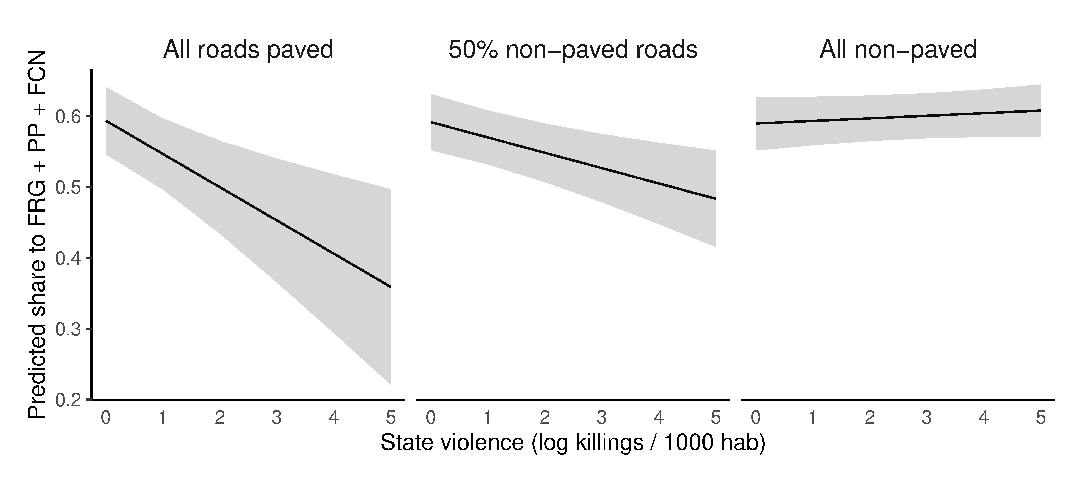
\includegraphics[width = 0.7\textwidth]{img/pp_fulldcha_roads}

  \caption{Wartime state violence and {\color{red}{\textbf{XXXXXXX}}} share depending on prewar political mobilization (proxied by \% non-paved roads)} \label{fig:pp_fulldcha_roads}

\end{figure*}

\begin{figure*}[htb!]
  \centering
    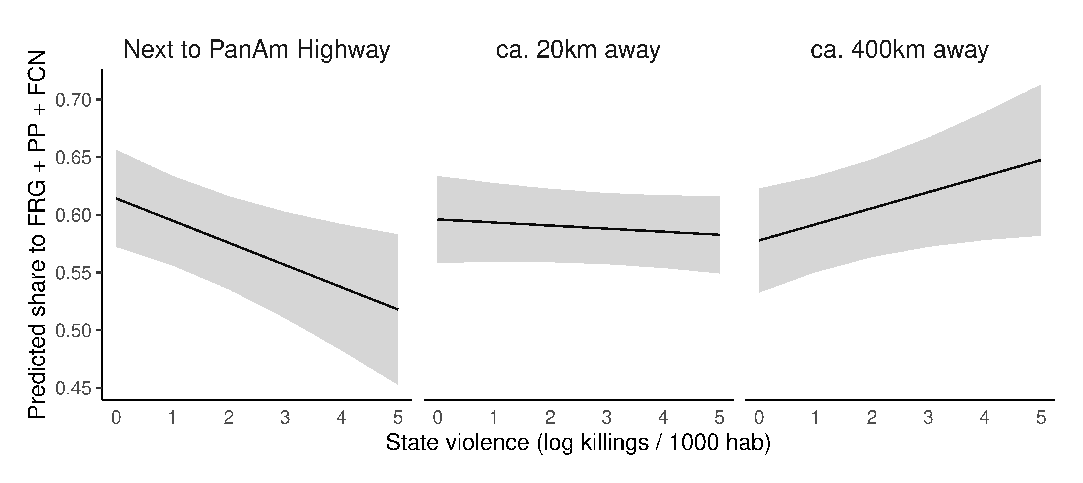
\includegraphics[width = 0.7\textwidth]{img/pp_fulldcha_panam}

  \caption{Wartime state violence and {\color{red}{\textbf{XXXXXXX}}} share depending on prewar political mobilization (proxied by distance to Pan-American Highway)} \label{fig:pp_fulldcha_panam}

\end{figure*}

\begin{figure*}[htb!]
  \centering
    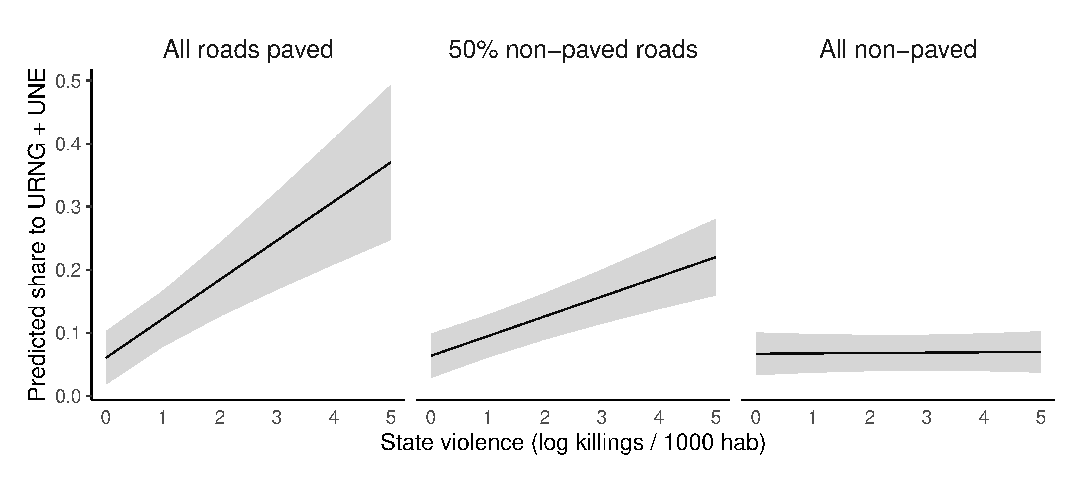
\includegraphics[width = 0.7\textwidth]{img/pp_fullizq_roads}

  \caption{Wartime state violence and {\color{red}{\textbf{XXXXXXX (izq)}}} share depending on prewar political mobilization (proxied by \% non-paved roads)} \label{fig:pp_fullizq_roads}

\end{figure*}

\begin{figure*}[htb!]
  \centering
    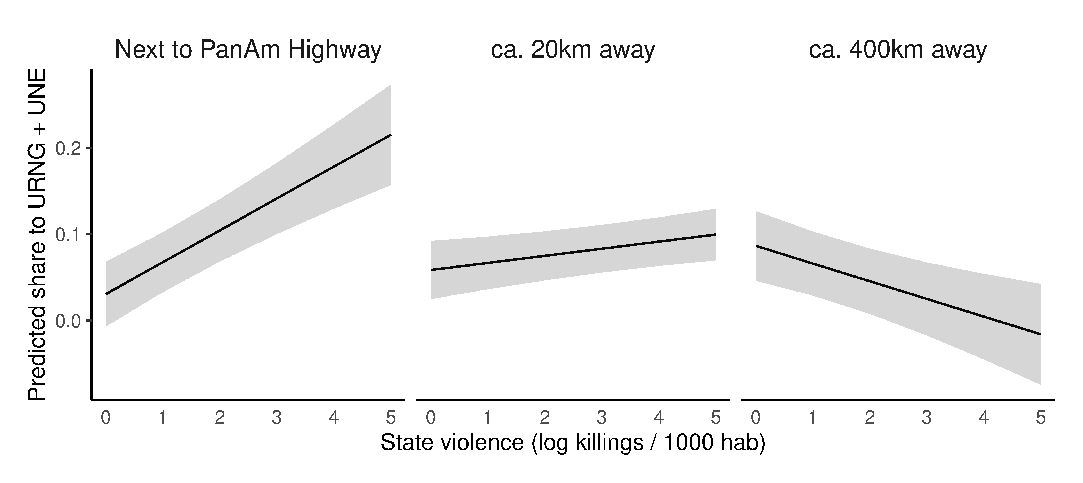
\includegraphics[width = 0.7\textwidth]{img/pp_fullizq_panam}

  \caption{Wartime state violence and {\color{red}{\textbf{XXXXXXX (izq)}}} share depending on prewar political mobilization (proxied by distance to Pan-American Highway)} \label{fig:pp_fullizq_panam}

\end{figure*}


\clearpage
\section{Results of cross-sectional models by election}\label{app:results_year}

Table \ref{tab:lm_URNG_roads_year}
Table \ref{tab:lm_URNG_panam_year}
Table \ref{tab:lm_URNG_base_year}
Table \ref{tab:lm_FRG_roads_year}
Table \ref{tab:lm_FRG_panam_year}
Table \ref{tab:lm_FRG_base_year}

Figure \ref{fig:pp_URNG_panam_yrs}
Figure \ref{fig:pp_URNG_roads_yrs}
Figure \ref{fig:pp_FRG_panam_yrs}
Figure \ref{fig:pp_FRG_roads_yrs}


% Table created by stargazer v.5.2.2 by Marek Hlavac, Harvard University. E-mail: hlavac at fas.harvard.edu
% Date and time: Tue, May 18, 2021 - 13:02:05
% Requires LaTeX packages: dcolumn 
\begin{table}[!htbp] \centering 
  \caption{Wartime violence and URNG share, by year (interaction, roads)} 
  \label{tab:lm_URNG_roads_year} 
\small 
\begin{tabular}{@{\extracolsep{-20pt}}lD{.}{.}{-3} D{.}{.}{-3} D{.}{.}{-3} D{.}{.}{-3} D{.}{.}{-3} } 
\\[-1.8ex]\hline 
\hline \\[-1.8ex] 
\\[-1.8ex] & \multicolumn{1}{c}{1999} & \multicolumn{1}{c}{2003} & \multicolumn{1}{c}{2007} & \multicolumn{1}{c}{2011} & \multicolumn{1}{c}{2015} \\ 
\\[-1.8ex] & \multicolumn{1}{c}{(1)} & \multicolumn{1}{c}{(2)} & \multicolumn{1}{c}{(3)} & \multicolumn{1}{c}{(4)} & \multicolumn{1}{c}{(5)}\\ 
\hline \\[-1.8ex] 
 (Intercept) & -0.230^{+} & -0.075 & -0.114^{+} & -0.166^{*} & -0.061 \\ 
  & (0.119) & (0.074) & (0.062) & (0.071) & (0.046) \\ 
  State-led killings & 0.116^{***} & 0.042^{**} & 0.021^{+} & 0.030^{*} & 0.018^{*} \\ 
  & (0.023) & (0.014) & (0.012) & (0.014) & (0.009) \\ 
  \% Non-paved roads & 0.013 & 0.006 & 0.008 & -0.002 & -0.007 \\ 
  & (0.028) & (0.017) & (0.015) & (0.017) & (0.011) \\ 
  Violence $\times$ Non-paved & -0.109^{***} & -0.044^{**} & -0.021 & -0.032^{*} & -0.019^{+} \\ 
  & (0.025) & (0.016) & (0.013) & (0.015) & (0.010) \\ 
  Log. Population 1973 & 0.015^{+} & 0.004 & 0.004 & 0.002 & -0.000 \\ 
  & (0.008) & (0.005) & (0.004) & (0.005) & (0.003) \\ 
  \% Indigenous 1973 & 0.095^{***} & 0.031^{*} & 0.026^{*} & 0.057^{***} & 0.027^{***} \\ 
  & (0.021) & (0.013) & (0.011) & (0.013) & (0.008) \\ 
  \% Literate 1973 & -0.000 & -0.000 & 0.000 & 0.000 & -0.000 \\ 
  & (0.000) & (0.000) & (0.000) & (0.000) & (0.000) \\ 
  Elevation SD & 0.023 & 0.024 & 0.007 & 0.017 & 0.004 \\ 
  & (0.025) & (0.016) & (0.013) & (0.015) & (0.009) \\ 
  Forest cover & 0.019 & 0.004 & 0.004 & 0.013 & 0.003 \\ 
  & (0.019) & (0.012) & (0.010) & (0.011) & (0.007) \\ 
  Log. Dist to capital & 0.011 & 0.002 & 0.004 & 0.008^{+} & 0.009^{**} \\ 
  & (0.008) & (0.005) & (0.004) & (0.005) & (0.003) \\ 
  Log. Area & -0.019 & 0.005 & 0.014 & 0.006 & 0.012 \\ 
  & (0.129) & (0.079) & (0.066) & (0.076) & (0.049) \\ 
 \hline \\[-1.8ex] 
Department FE & \multicolumn{1}{c}{Yes} & \multicolumn{1}{c}{Yes} & \multicolumn{1}{c}{Yes} & \multicolumn{1}{c}{Yes} & \multicolumn{1}{c}{Yes} \\ 
Observations & \multicolumn{1}{c}{325} & \multicolumn{1}{c}{318} & \multicolumn{1}{c}{323} & \multicolumn{1}{c}{320} & \multicolumn{1}{c}{315} \\ 
R$^{2}$ & \multicolumn{1}{c}{0.473} & \multicolumn{1}{c}{0.279} & \multicolumn{1}{c}{0.236} & \multicolumn{1}{c}{0.370} & \multicolumn{1}{c}{0.290} \\ 
Adjusted R$^{2}$ & \multicolumn{1}{c}{0.418} & \multicolumn{1}{c}{0.201} & \multicolumn{1}{c}{0.155} & \multicolumn{1}{c}{0.302} & \multicolumn{1}{c}{0.213} \\ 
\hline 
\hline \\[-1.8ex] 
\multicolumn{6}{c}{\parbox[t]{0.65\textwidth}{\textit{Note:} $+ p<0.1; * p<0.05; ** p<0.01; *** p<0.001$. Each model includes cross-sectional data on a specific election. Deparment FE not shown.}} \\ 
\end{tabular} 
\end{table} 


% Table created by stargazer v.5.2.2 by Marek Hlavac, Harvard University. E-mail: hlavac at fas.harvard.edu
% Date and time: Fri, Oct 29, 2021 - 20:39:04
% Requires LaTeX packages: dcolumn 
\begin{table}[!htbp] \centering 
  \caption{Wartime violence and URNG share, by year (interaction, PanAm)} 
  \label{tab:lm_URNG_panam_year} 
\small 
\begin{tabular}{@{\extracolsep{-20pt}}lD{.}{.}{-3} D{.}{.}{-3} D{.}{.}{-3} D{.}{.}{-3} D{.}{.}{-3} } 
\\[-1.8ex]\hline 
\hline \\[-1.8ex] 
\\[-1.8ex] & \multicolumn{1}{c}{1999} & \multicolumn{1}{c}{2003} & \multicolumn{1}{c}{2007} & \multicolumn{1}{c}{2011} & \multicolumn{1}{c}{2015} \\ 
\\[-1.8ex] & \multicolumn{1}{c}{(1)} & \multicolumn{1}{c}{(2)} & \multicolumn{1}{c}{(3)} & \multicolumn{1}{c}{(4)} & \multicolumn{1}{c}{(5)}\\ 
\hline \\[-1.8ex] 
 (Intercept) & -0.044 & 0.070 & -0.089 & -0.101 & -0.022 \\ 
  & (0.131) & (0.076) & (0.061) & (0.089) & (0.053) \\ 
  State-led killings & 0.063^{***} & 0.002 & 0.012^{*} & 0.017^{*} & 0.008^{+} \\ 
  & (0.011) & (0.007) & (0.006) & (0.007) & (0.004) \\ 
  Log. Dist to Pan-Am Hwy & 0.000 & 0.001 & 0.002 & 0.001 & 0.002 \\ 
  & (0.006) & (0.004) & (0.003) & (0.004) & (0.002) \\ 
  Violence $\times$ Dist to Pan-Am & -0.013^{***} & -0.001 & -0.003 & -0.005^{*} & -0.002^{+} \\ 
  & (0.003) & (0.002) & (0.002) & (0.002) & (0.001) \\ 
  Turnout & -0.069 & -0.061^{+} &  & -0.031 & -0.025 \\ 
  & (0.054) & (0.035) &  & (0.053) & (0.027) \\ 
  Log. Population 1973 & 0.005 & -0.004 & 0.003 & -0.001 & -0.001 \\ 
  & (0.009) & (0.005) & (0.004) & (0.005) & (0.003) \\ 
  \% Indigenous 1973 & 0.098^{***} & 0.022^{+} & 0.027^{*} & 0.058^{***} & 0.027^{***} \\ 
  & (0.021) & (0.012) & (0.011) & (0.013) & (0.008) \\ 
  \% Literate 1973 & -0.000 & -0.000 & 0.000 & 0.000 & -0.000 \\ 
  & (0.000) & (0.000) & (0.000) & (0.000) & (0.000) \\ 
  Elevation SD & 0.027 & 0.023 & 0.007 & 0.018 & 0.004 \\ 
  & (0.025) & (0.015) & (0.013) & (0.015) & (0.010) \\ 
  Forest cover & 0.010 & -0.007 & 0.001 & 0.009 & -0.000 \\ 
  & (0.020) & (0.011) & (0.010) & (0.012) & (0.008) \\ 
  Log. Dist to capital & 0.015^{+} & 0.007 & 0.006 & 0.009^{*} & 0.009^{**} \\ 
  & (0.008) & (0.005) & (0.004) & (0.005) & (0.003) \\ 
  Log. Area & 0.009 & 0.010 & 0.018 & 0.014 & 0.016 \\ 
  & (0.129) & (0.072) & (0.066) & (0.076) & (0.049) \\ 
 \hline \\[-1.8ex] 
Department FE & \multicolumn{1}{c}{Yes} & \multicolumn{1}{c}{Yes} & \multicolumn{1}{c}{Yes} & \multicolumn{1}{c}{Yes} & \multicolumn{1}{c}{Yes} \\ 
Observations & \multicolumn{1}{c}{325} & \multicolumn{1}{c}{261} & \multicolumn{1}{c}{323} & \multicolumn{1}{c}{320} & \multicolumn{1}{c}{315} \\ 
R$^{2}$ & \multicolumn{1}{c}{0.476} & \multicolumn{1}{c}{0.260} & \multicolumn{1}{c}{0.237} & \multicolumn{1}{c}{0.374} & \multicolumn{1}{c}{0.287} \\ 
Adjusted R$^{2}$ & \multicolumn{1}{c}{0.419} & \multicolumn{1}{c}{0.160} & \multicolumn{1}{c}{0.155} & \multicolumn{1}{c}{0.304} & \multicolumn{1}{c}{0.206} \\ 
\hline 
\hline \\[-1.8ex] 
\multicolumn{6}{c}{\parbox[t]{0.65\textwidth}{\textit{Note:} $+ p<0.1; * p<0.05; ** p<0.01; *** p<0.001$. Each model includes cross-sectional data on a specific election. Deparment FE not shown.}} \\ 
\end{tabular} 
\end{table} 


% Table created by stargazer v.5.2.2 by Marek Hlavac, Harvard University. E-mail: hlavac at fas.harvard.edu
% Date and time: Fri, Oct 29, 2021 - 20:39:03
% Requires LaTeX packages: dcolumn 
\begin{table}[!htbp] \centering 
  \caption{Wartime violence and URNG share, by year (base models)} 
  \label{tab:lm_URNG_base_year} 
\small 
\begin{tabular}{@{\extracolsep{-20pt}}lD{.}{.}{-3} D{.}{.}{-3} D{.}{.}{-3} D{.}{.}{-3} D{.}{.}{-3} } 
\\[-1.8ex]\hline 
\hline \\[-1.8ex] 
\\[-1.8ex] & \multicolumn{1}{c}{1999} & \multicolumn{1}{c}{2003} & \multicolumn{1}{c}{2007} & \multicolumn{1}{c}{2011} & \multicolumn{1}{c}{2015} \\ 
\\[-1.8ex] & \multicolumn{1}{c}{(1)} & \multicolumn{1}{c}{(2)} & \multicolumn{1}{c}{(3)} & \multicolumn{1}{c}{(4)} & \multicolumn{1}{c}{(5)}\\ 
\hline \\[-1.8ex] 
 (Intercept) & -0.072 & 0.077 & -0.085 & -0.092 & -0.020 \\ 
  & (0.136) & (0.076) & (0.062) & (0.090) & (0.054) \\ 
  State-led killings & 0.022^{***} & 0.000 & 0.003 & 0.002 & 0.002 \\ 
  & (0.006) & (0.003) & (0.003) & (0.003) & (0.002) \\ 
  Turnout & -0.061 & -0.057 &  & -0.033 & -0.028 \\ 
  & (0.056) & (0.035) &  & (0.052) & (0.027) \\ 
  Log. Population 1973 & 0.012 & -0.003 & 0.005 & 0.002 & -0.000 \\ 
  & (0.009) & (0.005) & (0.004) & (0.005) & (0.003) \\ 
  \% Indigenous 1973 & 0.084^{**} & 0.014 & 0.019 & 0.044^{**} & 0.024^{*} \\ 
  & (0.027) & (0.015) & (0.013) & (0.015) & (0.010) \\ 
  \% Literate 1973 & -0.045 & -0.029 & -0.024 & -0.045 & -0.010 \\ 
  & (0.050) & (0.029) & (0.025) & (0.029) & (0.019) \\ 
  Elevation SD & -0.000 & -0.000 & -0.000 & 0.000 & -0.000 \\ 
  & (0.000) & (0.000) & (0.000) & (0.000) & (0.000) \\ 
  Forest cover & 0.029 & 0.022 & 0.007 & 0.018 & 0.005 \\ 
  & (0.026) & (0.015) & (0.013) & (0.015) & (0.010) \\ 
  Log. Dist to capital & 0.008 & -0.006 & 0.002 & 0.009 & 0.001 \\ 
  & (0.019) & (0.010) & (0.010) & (0.011) & (0.007) \\ 
  Log. Area & 0.008 & 0.006 & 0.004 & 0.006 & 0.008^{*} \\ 
  & (0.008) & (0.005) & (0.004) & (0.005) & (0.003) \\ 
  Rebel violence pre-78 & -0.008 & 0.014 & 0.018 & 0.013 & 0.015 \\ 
  & (0.132) & (0.072) & (0.067) & (0.077) & (0.049) \\ 
 \hline \\[-1.8ex] 
Department FE & \multicolumn{1}{c}{Yes} & \multicolumn{1}{c}{Yes} & \multicolumn{1}{c}{Yes} & \multicolumn{1}{c}{Yes} & \multicolumn{1}{c}{Yes} \\ 
Observations & \multicolumn{1}{c}{325} & \multicolumn{1}{c}{261} & \multicolumn{1}{c}{323} & \multicolumn{1}{c}{320} & \multicolumn{1}{c}{315} \\ 
R$^{2}$ & \multicolumn{1}{c}{0.444} & \multicolumn{1}{c}{0.263} & \multicolumn{1}{c}{0.232} & \multicolumn{1}{c}{0.365} & \multicolumn{1}{c}{0.280} \\ 
Adjusted R$^{2}$ & \multicolumn{1}{c}{0.385} & \multicolumn{1}{c}{0.167} & \multicolumn{1}{c}{0.153} & \multicolumn{1}{c}{0.297} & \multicolumn{1}{c}{0.201} \\ 
\hline 
\hline \\[-1.8ex] 
\multicolumn{6}{c}{\parbox[t]{0.65\textwidth}{\textit{Note:} $+ p<0.1; * p<0.05; ** p<0.01; *** p<0.001$. Each model includes cross-sectional data on a specific election. Deparment FE not shown.}} \\ 
\end{tabular} 
\end{table} 


% Table created by stargazer v.5.2.2 by Marek Hlavac, Harvard University. E-mail: hlavac at fas.harvard.edu
% Date and time: Mon, Jul 26, 2021 - 13:55:26
% Requires LaTeX packages: dcolumn 
\begin{table}[!htbp] \centering 
  \caption{Wartime violence and FRG share, by year (interaction, roads)} 
  \label{tab:lm_FRG_roads_year} 
\small 
\begin{tabular}{@{\extracolsep{-20pt}}lD{.}{.}{-3} D{.}{.}{-3} D{.}{.}{-3} D{.}{.}{-3} } 
\\[-1.8ex]\hline 
\hline \\[-1.8ex] 
\\[-1.8ex] & \multicolumn{1}{c}{1999} & \multicolumn{1}{c}{2003} & \multicolumn{1}{c}{2007} & \multicolumn{1}{c}{2015} \\ 
\\[-1.8ex] & \multicolumn{1}{c}{(1)} & \multicolumn{1}{c}{(2)} & \multicolumn{1}{c}{(3)} & \multicolumn{1}{c}{(4)}\\ 
\hline \\[-1.8ex] 
 (Intercept) & 0.684^{***} & 0.263 & 0.147 & 0.037^{*} \\ 
  & (0.179) & (0.171) & (0.101) & (0.017) \\ 
  State-led killings & -0.103^{***} & 0.015 & -0.026 & 0.000 \\ 
  & (0.031) & (0.029) & (0.019) & (0.003) \\ 
  \% Non-paved roads & -0.015 & 0.058 & 0.004 & -0.006^{+} \\ 
  & (0.037) & (0.036) & (0.024) & (0.003) \\ 
  Violence $\times$ Non-paved & 0.107^{**} & -0.016 & 0.033 & 0.000 \\ 
  & (0.034) & (0.032) & (0.022) & (0.003) \\ 
  Turnout & -0.124^{+} & 0.043 &  & -0.027^{**} \\ 
  & (0.073) & (0.078) &  & (0.009) \\ 
  Log. Population 1973 & 0.010 & -0.020^{+} & 0.000 & -0.001 \\ 
  & (0.012) & (0.011) & (0.007) & (0.001) \\ 
  \% Indigenous 1973 & -0.098^{***} & 0.038 & 0.014 & 0.003 \\ 
  & (0.028) & (0.027) & (0.018) & (0.003) \\ 
  \% Literate 1973 & -0.000^{+} & 0.000 & -0.000 & 0.000 \\ 
  & (0.000) & (0.000) & (0.000) & (0.000) \\ 
  Elevation SD & -0.038 & -0.044 & -0.019 & -0.001 \\ 
  & (0.033) & (0.033) & (0.021) & (0.003) \\ 
  Forest cover & 0.013 & 0.003 & -0.011 & -0.001 \\ 
  & (0.026) & (0.023) & (0.016) & (0.002) \\ 
  Log. Dist to capital & -0.013 & 0.009 & 0.009 & 0.000 \\ 
  & (0.011) & (0.010) & (0.007) & (0.001) \\ 
  Log. Area & 0.068 & 0.055 & -0.031 & -0.004 \\ 
  & (0.172) & (0.157) & (0.109) & (0.015) \\ 
 \hline \\[-1.8ex] 
Department FE & \multicolumn{1}{c}{Yes} & \multicolumn{1}{c}{Yes} & \multicolumn{1}{c}{Yes} & \multicolumn{1}{c}{Yes} \\ 
Observations & \multicolumn{1}{c}{325} & \multicolumn{1}{c}{261} & \multicolumn{1}{c}{323} & \multicolumn{1}{c}{315} \\ 
R$^{2}$ & \multicolumn{1}{c}{0.319} & \multicolumn{1}{c}{0.378} & \multicolumn{1}{c}{0.393} & \multicolumn{1}{c}{0.208} \\ 
Adjusted R$^{2}$ & \multicolumn{1}{c}{0.245} & \multicolumn{1}{c}{0.294} & \multicolumn{1}{c}{0.328} & \multicolumn{1}{c}{0.118} \\ 
\hline 
\hline \\[-1.8ex] 
\multicolumn{5}{c}{\parbox[t]{0.65\textwidth}{\textit{Note:} $+ p<0.1; * p<0.05; ** p<0.01; *** p<0.001$. Each model includes cross-sectional data on a specific election. Deparment FE not shown.}} \\ 
\end{tabular} 
\end{table} 


% Table created by stargazer v.5.2.2 by Marek Hlavac, Harvard University. E-mail: hlavac at fas.harvard.edu
% Date and time: Fri, Oct 29, 2021 - 20:39:05
% Requires LaTeX packages: dcolumn 
\begin{table}[!htbp] \centering 
  \caption{Wartime violence and FRG share, by year (interaction, PanAm)} 
  \label{tab:lm_FRG_panam_year} 
\small 
\begin{tabular}{@{\extracolsep{-20pt}}lD{.}{.}{-3} D{.}{.}{-3} D{.}{.}{-3} D{.}{.}{-3} } 
\\[-1.8ex]\hline 
\hline \\[-1.8ex] 
\\[-1.8ex] & \multicolumn{1}{c}{1999} & \multicolumn{1}{c}{2003} & \multicolumn{1}{c}{2007} & \multicolumn{1}{c}{2015} \\ 
\\[-1.8ex] & \multicolumn{1}{c}{(1)} & \multicolumn{1}{c}{(2)} & \multicolumn{1}{c}{(3)} & \multicolumn{1}{c}{(4)}\\ 
\hline \\[-1.8ex] 
 (Intercept) & 0.567^{**} & 0.308^{+} & 0.131 & 0.034^{*} \\ 
  & (0.177) & (0.165) & (0.100) & (0.017) \\ 
  State-led killings & -0.038^{*} & 0.015 & 0.005 & 0.003^{*} \\ 
  & (0.015) & (0.015) & (0.010) & (0.001) \\ 
  Log. Dist to Pan-Am Hwy & -0.007 & 0.017^{*} & 0.006 & -0.001 \\ 
  & (0.008) & (0.008) & (0.005) & (0.001) \\ 
  Violence $\times$ Dist to Pan-Am & 0.009^{*} & -0.005 & -0.001 & -0.001 \\ 
  & (0.004) & (0.004) & (0.003) & (0.000) \\ 
  Turnout & -0.103 & 0.054 &  & -0.027^{**} \\ 
  & (0.073) & (0.077) &  & (0.008) \\ 
  Log. Population 1973 & 0.015 & -0.024^{*} & 0.001 & -0.001 \\ 
  & (0.012) & (0.010) & (0.007) & (0.001) \\ 
  \% Indigenous 1973 & -0.101^{***} & 0.040 & 0.015 & 0.002 \\ 
  & (0.028) & (0.027) & (0.018) & (0.002) \\ 
  \% Literate 1973 & -0.000 & -0.000 & -0.000 & 0.000^{+} \\ 
  & (0.000) & (0.000) & (0.000) & (0.000) \\ 
  Elevation SD & -0.040 & -0.050 & -0.024 & -0.001 \\ 
  & (0.034) & (0.033) & (0.021) & (0.003) \\ 
  Forest cover & 0.029 & -0.008 & -0.013 & 0.000 \\ 
  & (0.027) & (0.024) & (0.017) & (0.002) \\ 
  Log. Dist to capital & -0.016 & 0.014 & 0.010 & 0.000 \\ 
  & (0.011) & (0.010) & (0.007) & (0.001) \\ 
  Log. Area & 0.050 & 0.066 & -0.036 & -0.001 \\ 
  & (0.174) & (0.157) & (0.109) & (0.015) \\ 
 \hline \\[-1.8ex] 
Department FE & \multicolumn{1}{c}{Yes} & \multicolumn{1}{c}{Yes} & \multicolumn{1}{c}{Yes} & \multicolumn{1}{c}{Yes} \\ 
Observations & \multicolumn{1}{c}{325} & \multicolumn{1}{c}{261} & \multicolumn{1}{c}{323} & \multicolumn{1}{c}{315} \\ 
R$^{2}$ & \multicolumn{1}{c}{0.306} & \multicolumn{1}{c}{0.383} & \multicolumn{1}{c}{0.390} & \multicolumn{1}{c}{0.217} \\ 
Adjusted R$^{2}$ & \multicolumn{1}{c}{0.230} & \multicolumn{1}{c}{0.300} & \multicolumn{1}{c}{0.325} & \multicolumn{1}{c}{0.128} \\ 
\hline 
\hline \\[-1.8ex] 
\multicolumn{5}{c}{\parbox[t]{0.65\textwidth}{\textit{Note:} $+ p<0.1; * p<0.05; ** p<0.01; *** p<0.001$. Each model includes cross-sectional data on a specific election. Deparment FE not shown.}} \\ 
\end{tabular} 
\end{table} 


% Table created by stargazer v.5.2.2 by Marek Hlavac, Harvard University. E-mail: hlavac at fas.harvard.edu
% Date and time: Fri, Jul 02, 2021 - 12:56:10
% Requires LaTeX packages: dcolumn 
\begin{table}[!htbp] \centering 
  \caption{Wartime violence and FRG share, by year (base models)} 
  \label{tab:lm_FRG_base_year} 
\small 
\begin{tabular}{@{\extracolsep{-20pt}}lD{.}{.}{-3} D{.}{.}{-3} D{.}{.}{-3} D{.}{.}{-3} } 
\\[-1.8ex]\hline 
\hline \\[-1.8ex] 
\\[-1.8ex] & \multicolumn{1}{c}{1999} & \multicolumn{1}{c}{2003} & \multicolumn{1}{c}{2007} & \multicolumn{1}{c}{2015} \\ 
\\[-1.8ex] & \multicolumn{1}{c}{(1)} & \multicolumn{1}{c}{(2)} & \multicolumn{1}{c}{(3)} & \multicolumn{1}{c}{(4)}\\ 
\hline \\[-1.8ex] 
 (Intercept) & 0.516^{**} & 0.362^{*} & 0.143 & 0.030^{+} \\ 
  & (0.176) & (0.164) & (0.102) & (0.017) \\ 
  State-led killings & -0.010 & -0.000 & 0.002 & 0.001 \\ 
  & (0.008) & (0.007) & (0.005) & (0.001) \\ 
  Turnout & -0.129^{+} & 0.073 &  & -0.028^{**} \\ 
  & (0.073) & (0.077) &  & (0.008) \\ 
  Log. Population 1973 & 0.005 & -0.019^{+} & 0.001 & -0.001 \\ 
  & (0.011) & (0.010) & (0.007) & (0.001) \\ 
  \% Indigenous 1973 & -0.035 & -0.011 & 0.006 & 0.004 \\ 
  & (0.035) & (0.032) & (0.022) & (0.003) \\ 
  \% Literate 1973 & 0.206^{**} & -0.179^{**} & -0.026 & 0.006 \\ 
  & (0.065) & (0.062) & (0.041) & (0.006) \\ 
  Elevation SD & -0.000 & -0.000 & -0.000 & 0.000 \\ 
  & (0.000) & (0.000) & (0.000) & (0.000) \\ 
  Forest cover & -0.038 & -0.052 & -0.022 & -0.001 \\ 
  & (0.033) & (0.033) & (0.021) & (0.003) \\ 
  Log. Dist to capital & 0.024 & 0.008 & -0.007 & -0.001 \\ 
  & (0.025) & (0.022) & (0.016) & (0.002) \\ 
  Log. Area & -0.005 & 0.006 & 0.009 & 0.000 \\ 
  & (0.011) & (0.010) & (0.007) & (0.001) \\ 
  Rebel violence pre-78 & 0.034 & 0.087 & -0.031 & -0.004 \\ 
  & (0.172) & (0.156) & (0.109) & (0.015) \\ 
 \hline \\[-1.8ex] 
Department FE & \multicolumn{1}{c}{Yes} & \multicolumn{1}{c}{Yes} & \multicolumn{1}{c}{Yes} & \multicolumn{1}{c}{Yes} \\ 
Observations & \multicolumn{1}{c}{325} & \multicolumn{1}{c}{261} & \multicolumn{1}{c}{323} & \multicolumn{1}{c}{315} \\ 
R$^{2}$ & \multicolumn{1}{c}{0.319} & \multicolumn{1}{c}{0.393} & \multicolumn{1}{c}{0.388} & \multicolumn{1}{c}{0.201} \\ 
Adjusted R$^{2}$ & \multicolumn{1}{c}{0.247} & \multicolumn{1}{c}{0.314} & \multicolumn{1}{c}{0.325} & \multicolumn{1}{c}{0.114} \\ 
\hline 
\hline \\[-1.8ex] 
\multicolumn{5}{c}{\parbox[t]{0.65\textwidth}{\textit{Note:} $+ p<0.1; * p<0.05; ** p<0.01; *** p<0.001$. Each model includes cross-sectional data on a specific election. Deparment FE not shown.}} \\ 
\end{tabular} 
\end{table} 



\begin{figure*}[htb!]
  \centering
    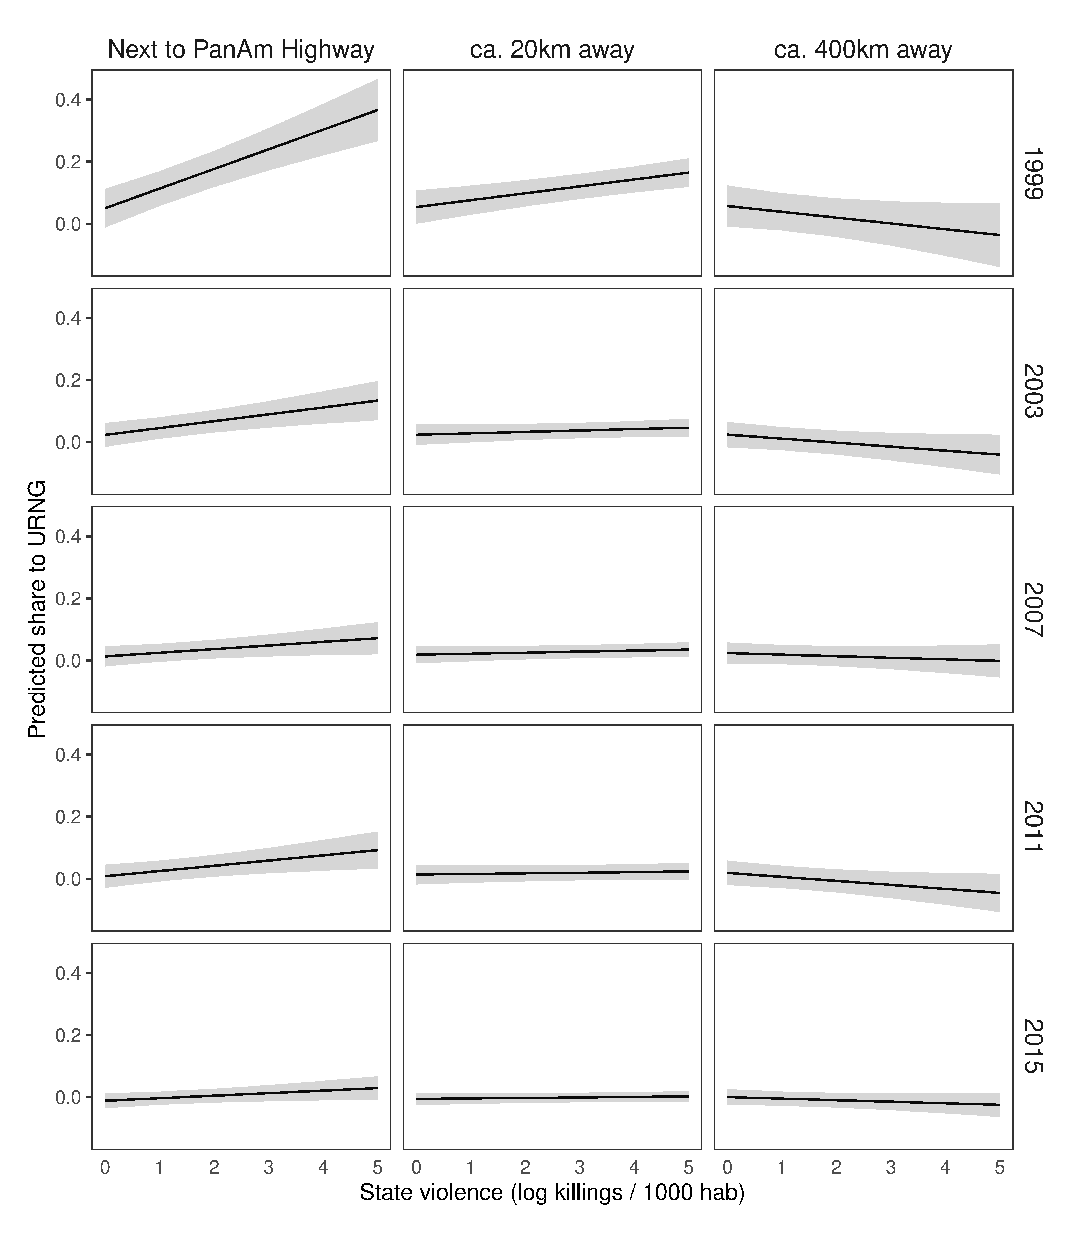
\includegraphics[width = \textwidth]{img/pp_URNG_panam_year}

  \caption{Wartime state violence and URNG share depending on prewar political mobilization (proxied by distance to Pan-American Highway)} \label{fig:pp_URNG_panam_yrs}

\end{figure*}

\begin{figure*}[htb!]
  \centering
    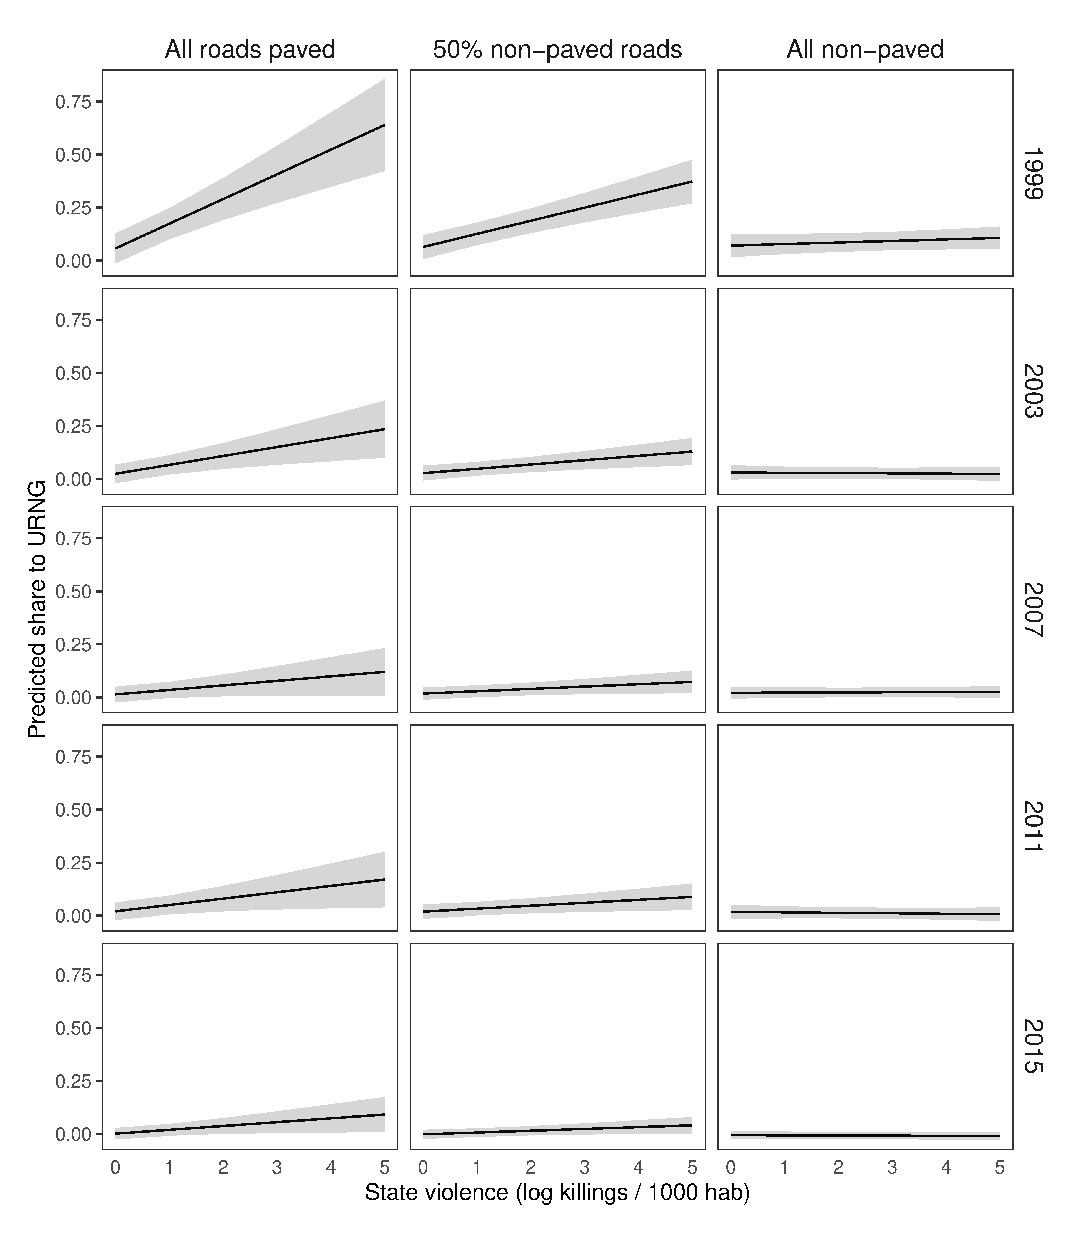
\includegraphics[width = \textwidth]{img/pp_URNG_roads_year}

  \caption{Wartime state violence and URNG share depending on prewar political mobilization (proxied by \% non-paved roads)} \label{fig:pp_URNG_roads_yrs}

\end{figure*}

\begin{figure*}[htb!]
  \centering
    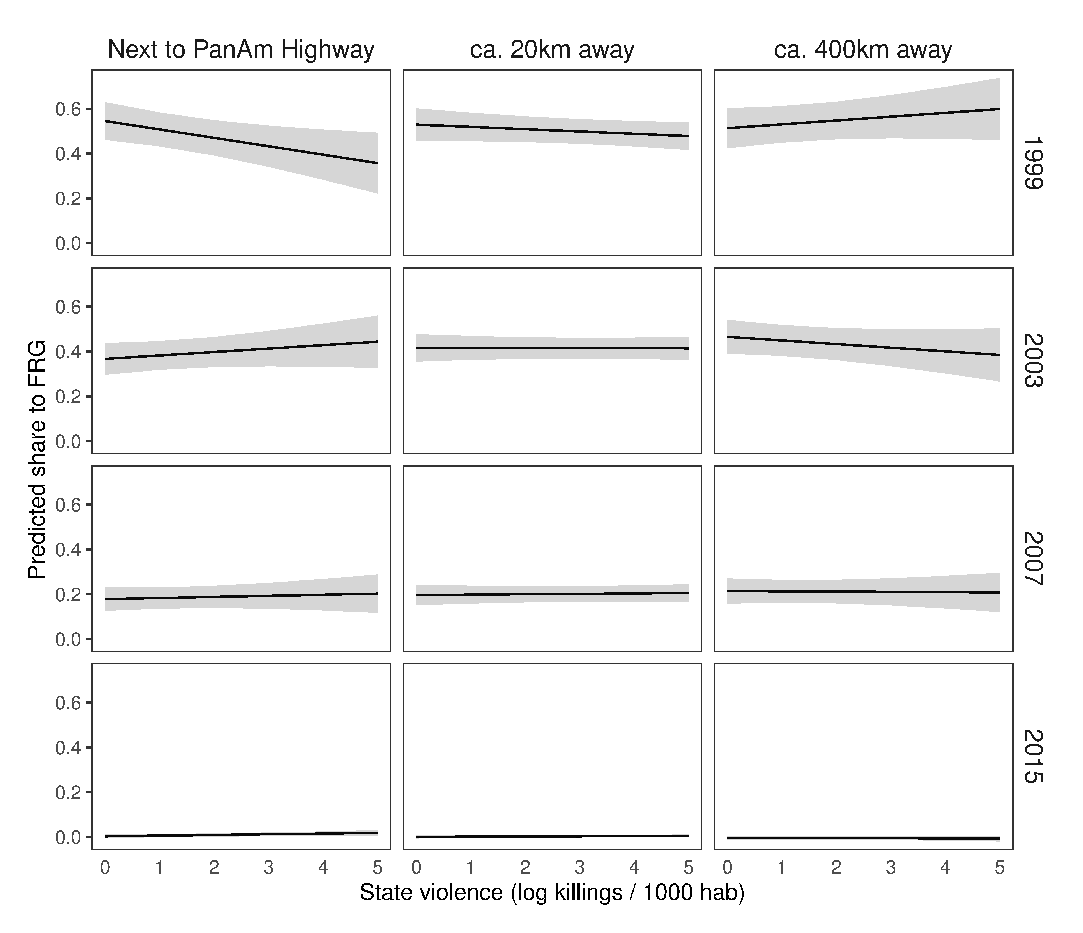
\includegraphics[width = 0.7\textwidth]{img/pp_FRG_panam_year}

  \caption{Wartime state violence and FRG share depending on prewar political mobilization (proxied by distance to Pan-American Highway)} \label{fig:pp_FRG_panam_yrs}

\end{figure*}

\begin{figure*}[htb!]
  \centering
    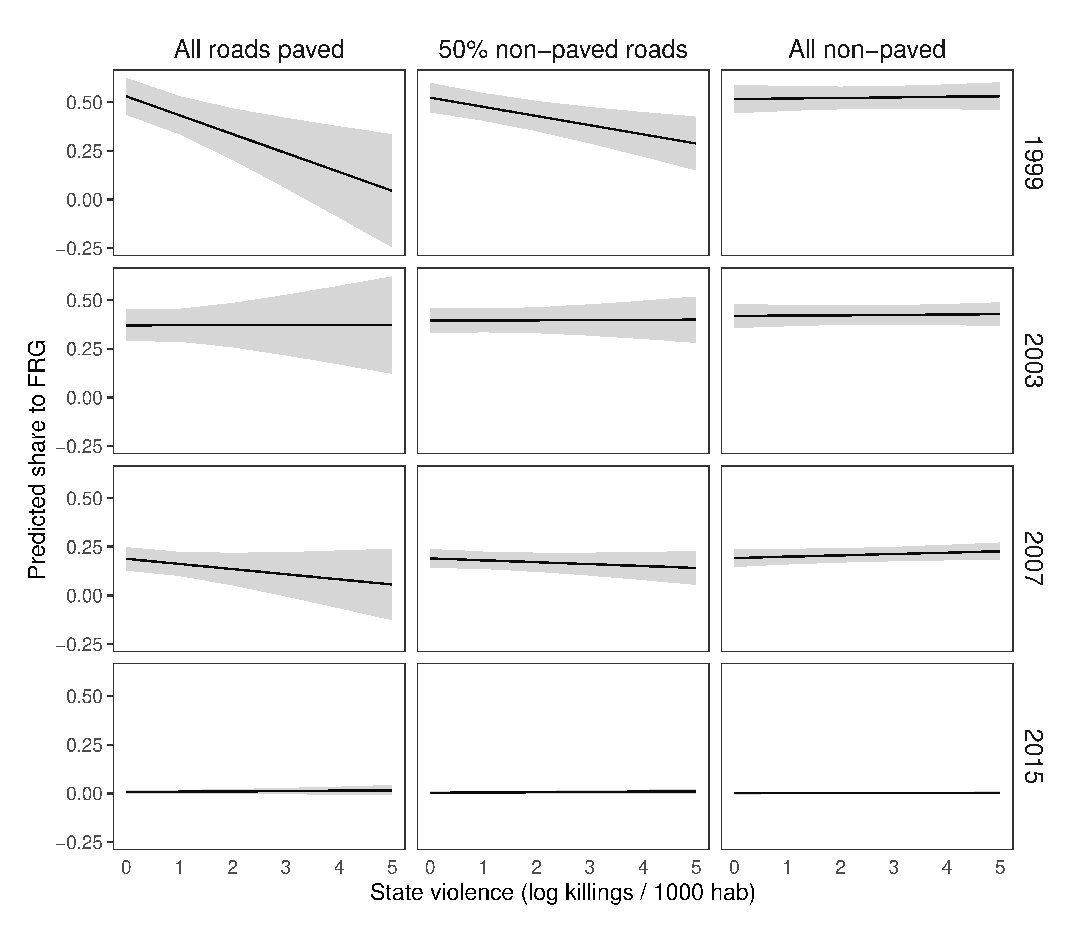
\includegraphics[width = 0.7\textwidth]{img/pp_FRG_roads_year}

  \caption{Wartime state violence and FRG share depending on prewar political mobilization (proxied by \% non-paved roads)} \label{fig:pp_FRG_roads_yrs}

\end{figure*}

\end{document}
